
\begin{figure*}[ht!]
	\centering
	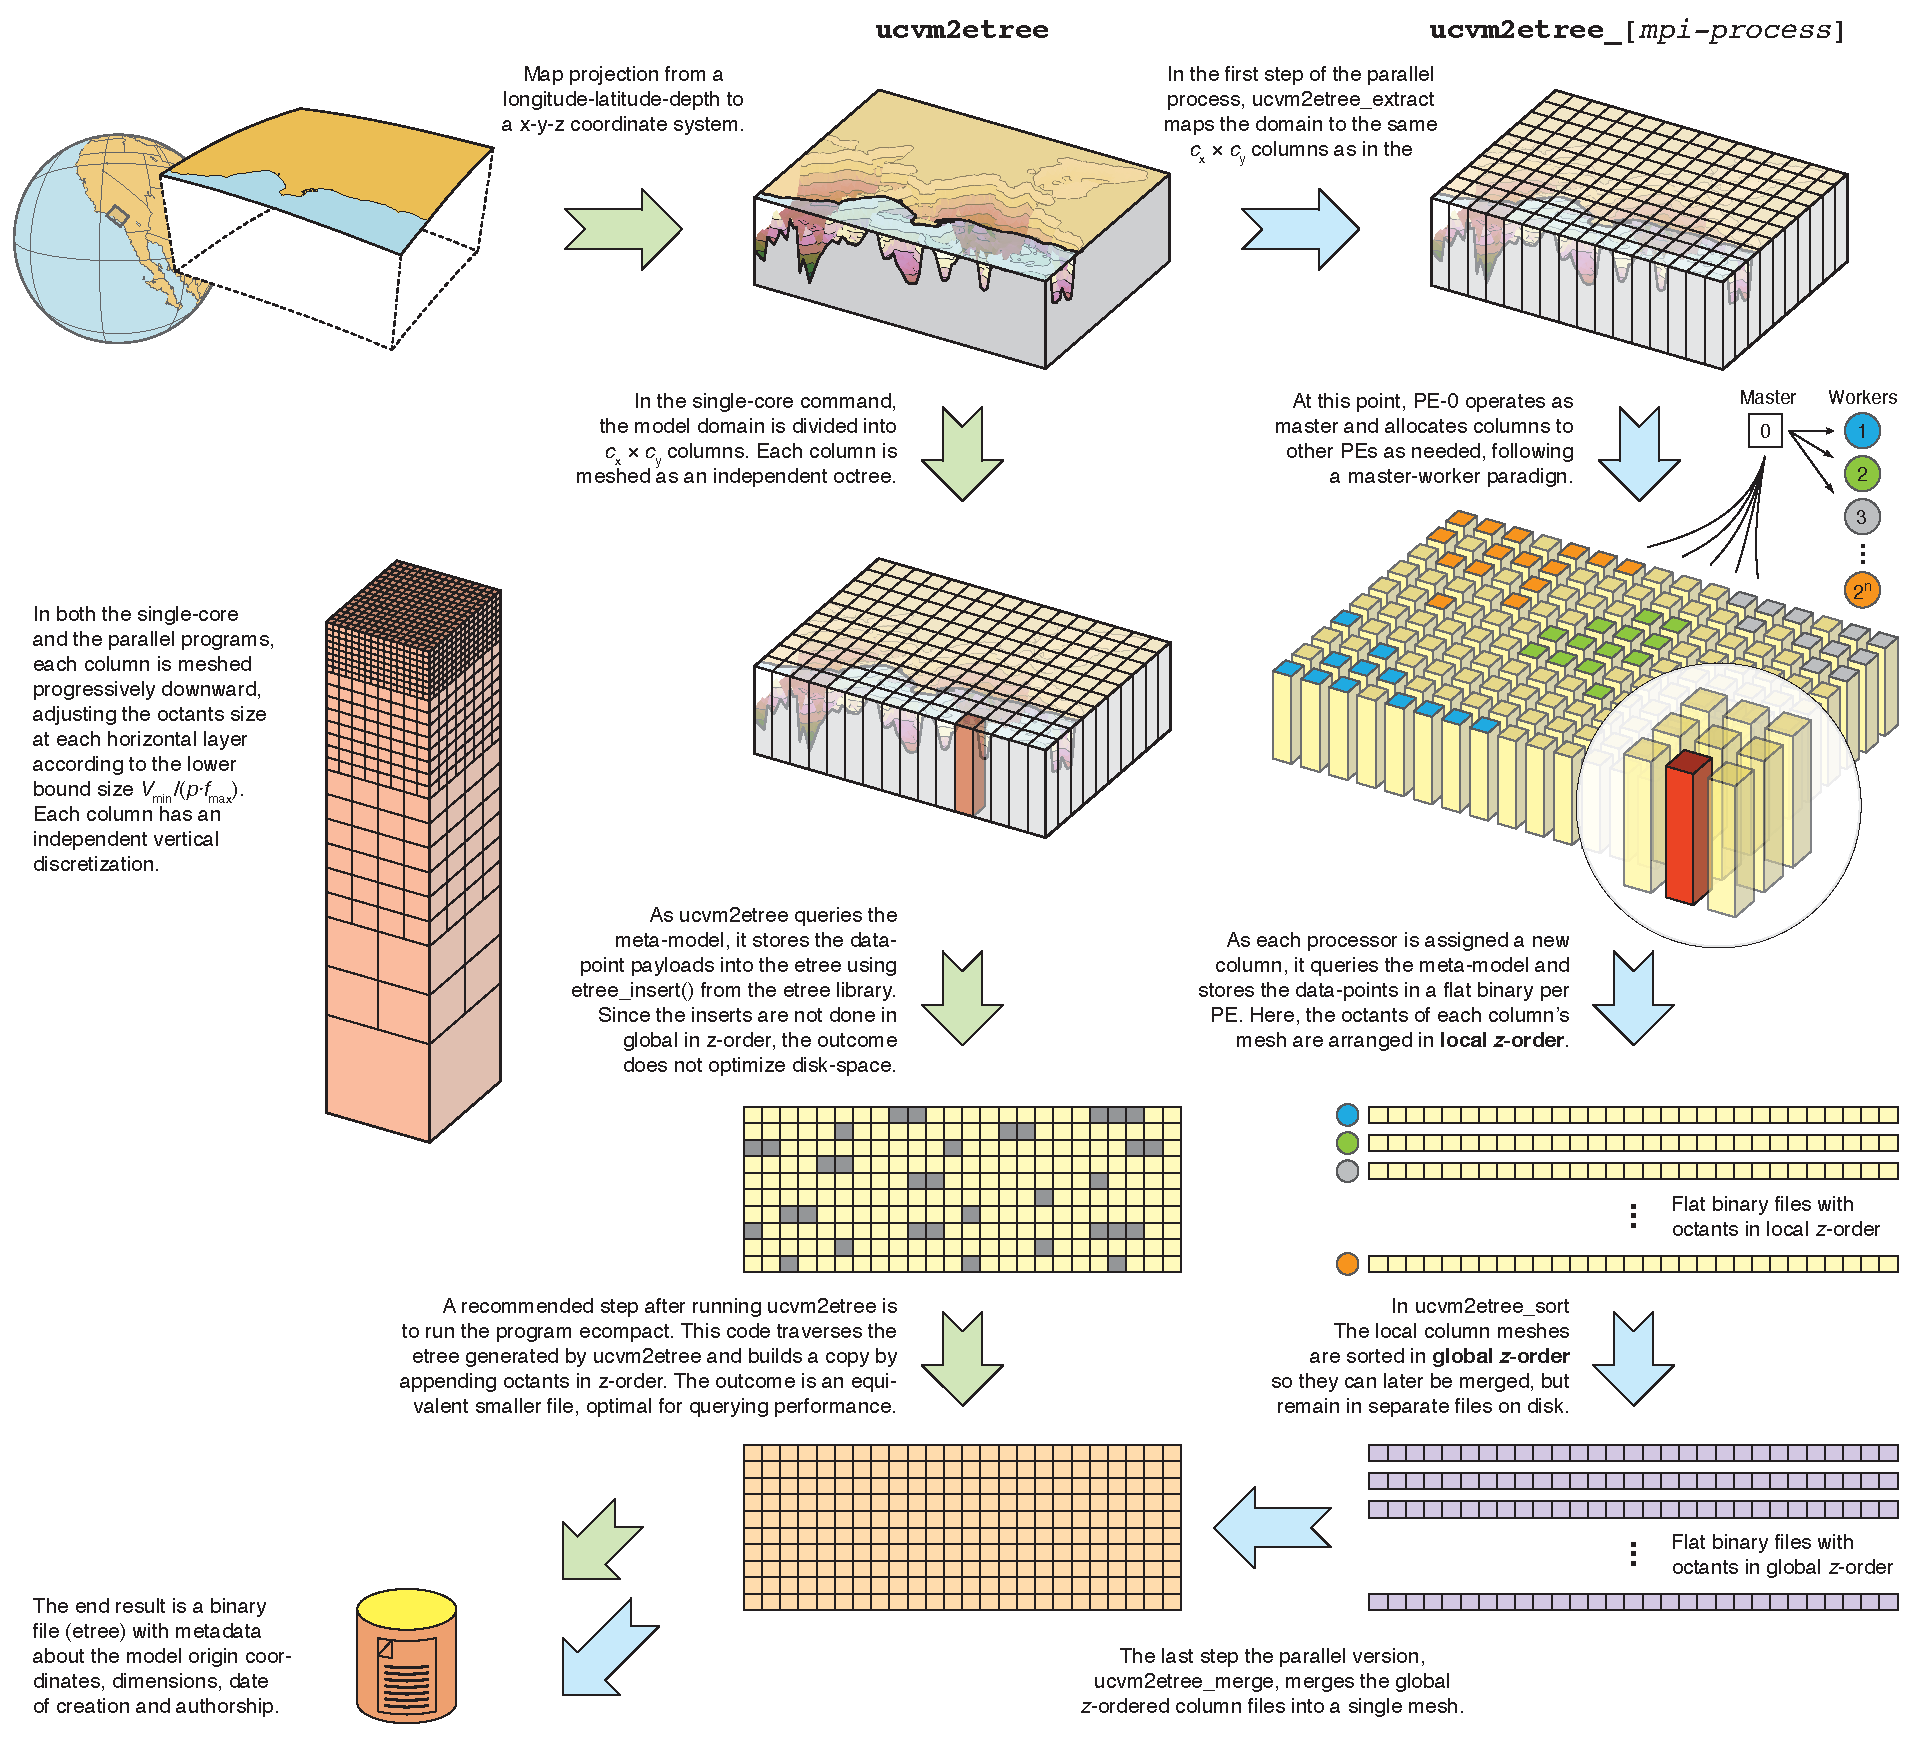
\includegraphics
		[width=\textwidth]
		{figures/pdf/ucvm-to-etree}
	\caption{Construction of an semi-unstructured mesh in the etree database format using the program \texttt{ucvm2etree} (green arrows); and its MPI equivalent process controlled by the programs \texttt{ucvm2etree\_extract}, \texttt{ucvm2etree\_sort} and \texttt{ucvm2etree\_merge} (blue arrows). Note that the information payload (\vs{}, \vp{}, and $\rho$) is associated with the octants in the octree structure and not with a point. In other words, the querying and assignment process maps the information queried at the center of each octant to the whole volume enclosed by the octant.}
	\label{fig:etrees}
\end{figure*}
% ---------------------------------------------------------------------------------------------
